% Adjust these for the path of the theme and its graphics, relative to this file
%\usepackage{beamerthemeFalmouthGamesAcademy}
\usepackage{../../beamerthemeFalmouthGamesAcademy}
\usepackage{multimedia}
\graphicspath{ {../../} }

% Default language for code listings
\lstset{language=C++,
        morekeywords={each,in,nullptr}
}

% For strikethrough effect
\usepackage[normalem]{ulem}
\usepackage{wasysym}

\usepackage{pdfpages}

% http://www.texample.net/tikz/examples/state-machine/
\usetikzlibrary{arrows,automata}

\newcommand{\modulecode}{COMP260}\newcommand{\moduletitle}{Distributed Systems}\newcommand{\sessionnumber}{5}

\begin{document}
\title{\sessionnumber: GPU Optimisation}
\subtitle{\modulecode: \moduletitle}

\frame{\titlepage} 

\begin{frame}
	\frametitle{Learning outcomes}
	By the end of today's session, you will be able to:
	\begin{itemize}
		\item \textbf{Recall} the key stages of the graphics pipeline
		\item \textbf{Understand} the GPU Debugger 
		\item \textbf{Explain} some of the key areas for optimisation
	\end{itemize}
\end{frame}

%Add in the other shader stages(Tesselation and Geometry)
\part{The 3D graphics pipeline}
\frame{\partpage}

\begin{frame}{The 3D graphics pipeline}
	\begin{center}
		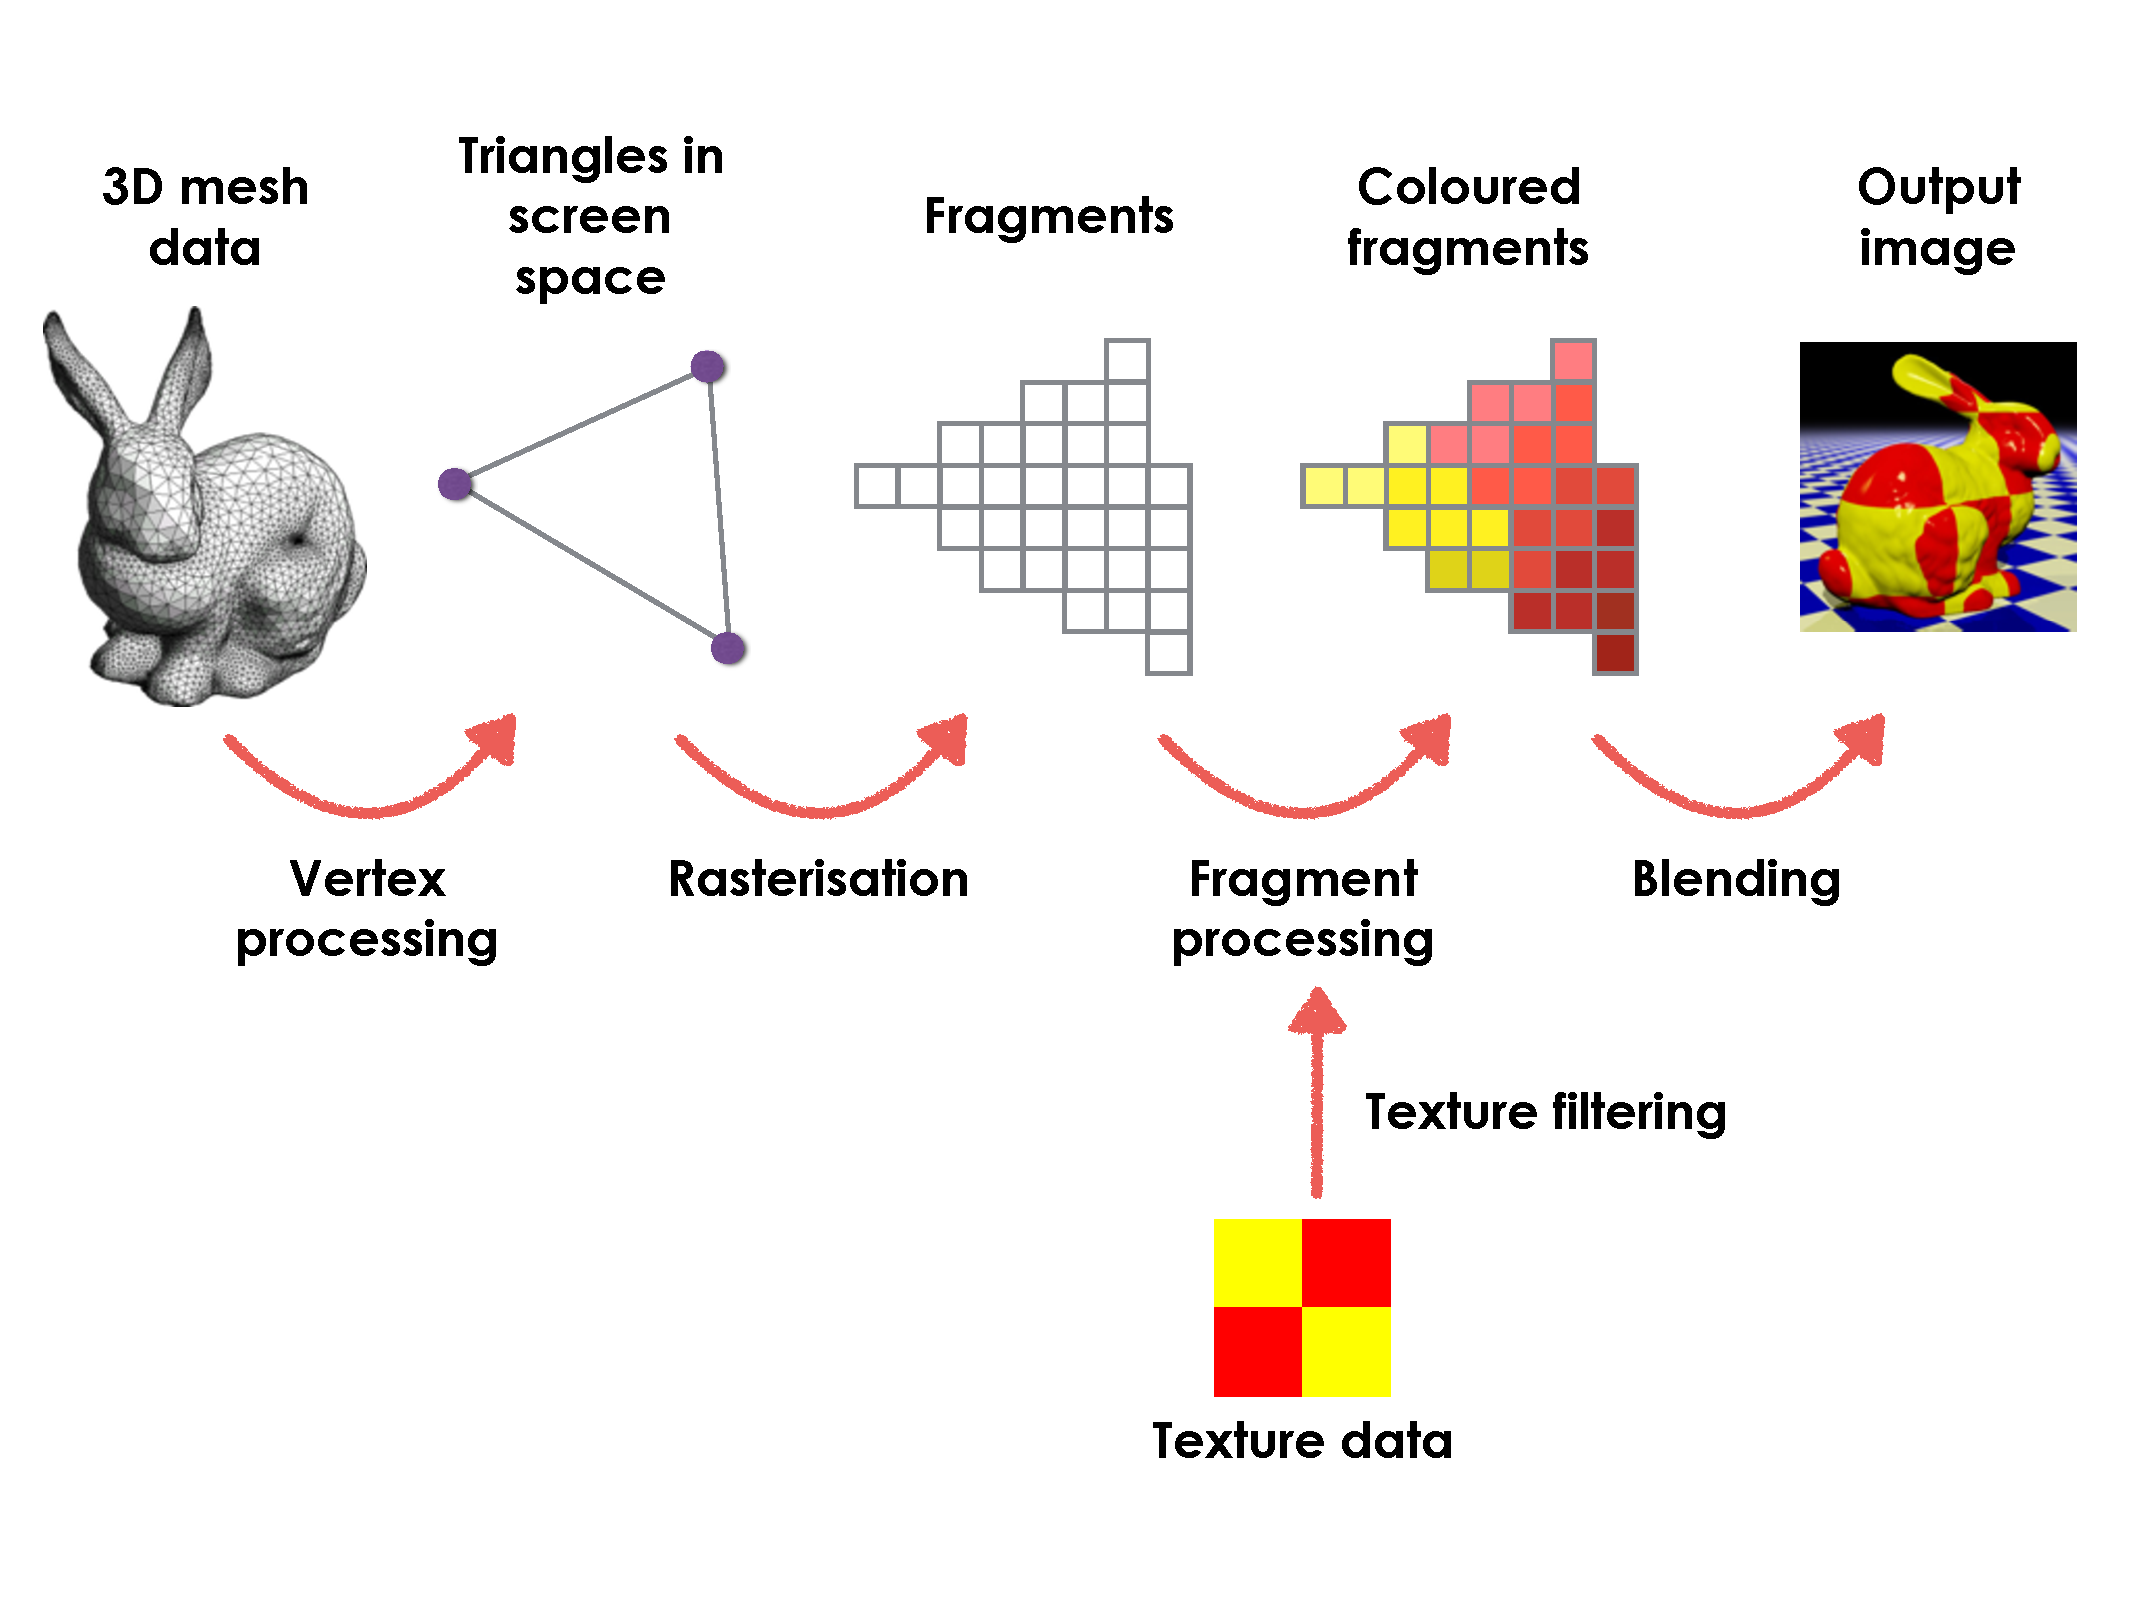
\includegraphics[height=0.7\textheight]{pipeline}
	\end{center}
\end{frame}

\begin{frame}{Vertex processing}
	\begin{columns}
		\begin{column}{0.3\textwidth}
			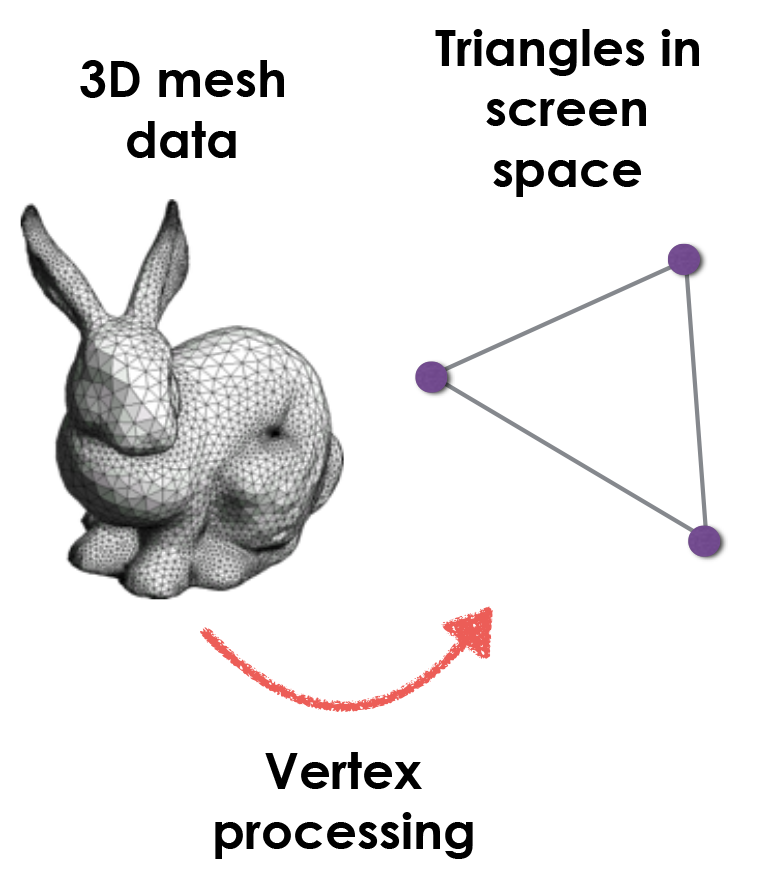
\includegraphics[width=\textwidth]{pipeline_1}
		\end{column}
		\begin{column}{0.65\textwidth}
			\begin{itemize}
				\pause\item Geometry is provided to the GPU as a \textbf{mesh} of \textbf{triangles}
				\pause\item Each triangle has three \textbf{vertices} specified in 3D space $(x,y,z)$
				\pause\item Vertex processor \textbf{transforms} (rotates, moves, scales) vertices
					and \textbf{projects} them into 2D screen space $(x,y)$
				\pause\item May also apply particle simulations, skeletal animations or deformations, etc.
			\end{itemize}
		\end{column}
	\end{columns}
\end{frame}

\begin{frame}{Rasterisation}
	\begin{columns}
		\begin{column}{0.3\textwidth}
			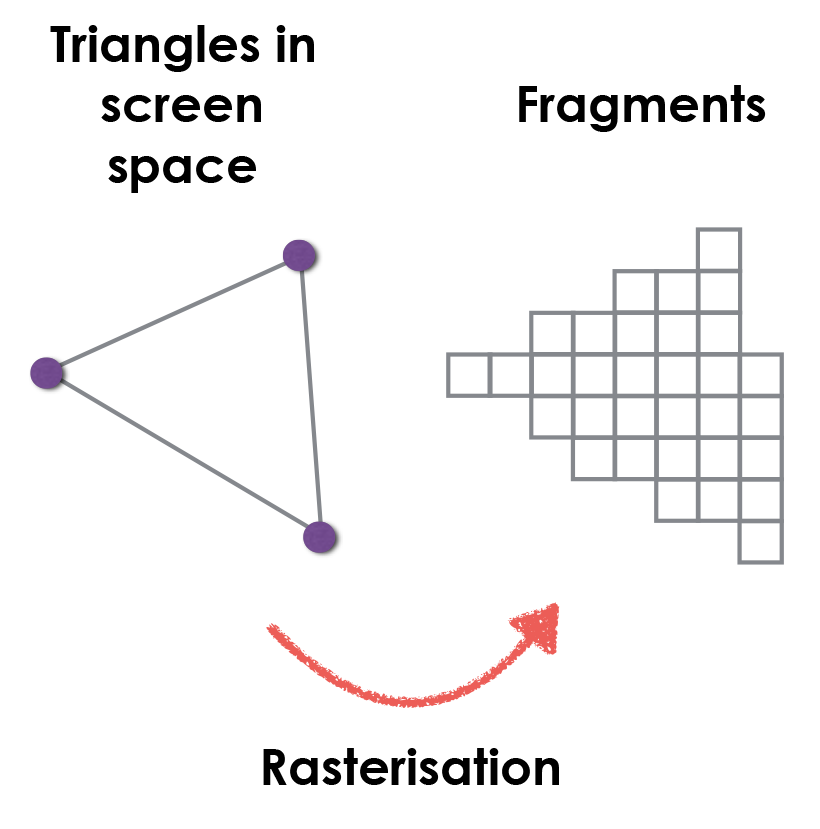
\includegraphics[width=\textwidth]{pipeline_2}
		\end{column}
		\begin{column}{0.65\textwidth}
			\begin{itemize}
				\pause\item Determine \textbf{which fragments} are covered by the triangle
				\pause\item In practical terms, ``fragment'' = ``pixel''
				\pause\item Vertex processor can associate \textbf{data} with each vertex;
					this is \textbf{interpolated} across the fragments
			\end{itemize}
		\end{column}
	\end{columns}
\end{frame}

\begin{frame}{Fragment processing}
	\begin{columns}
		\begin{column}{0.3\textwidth}
			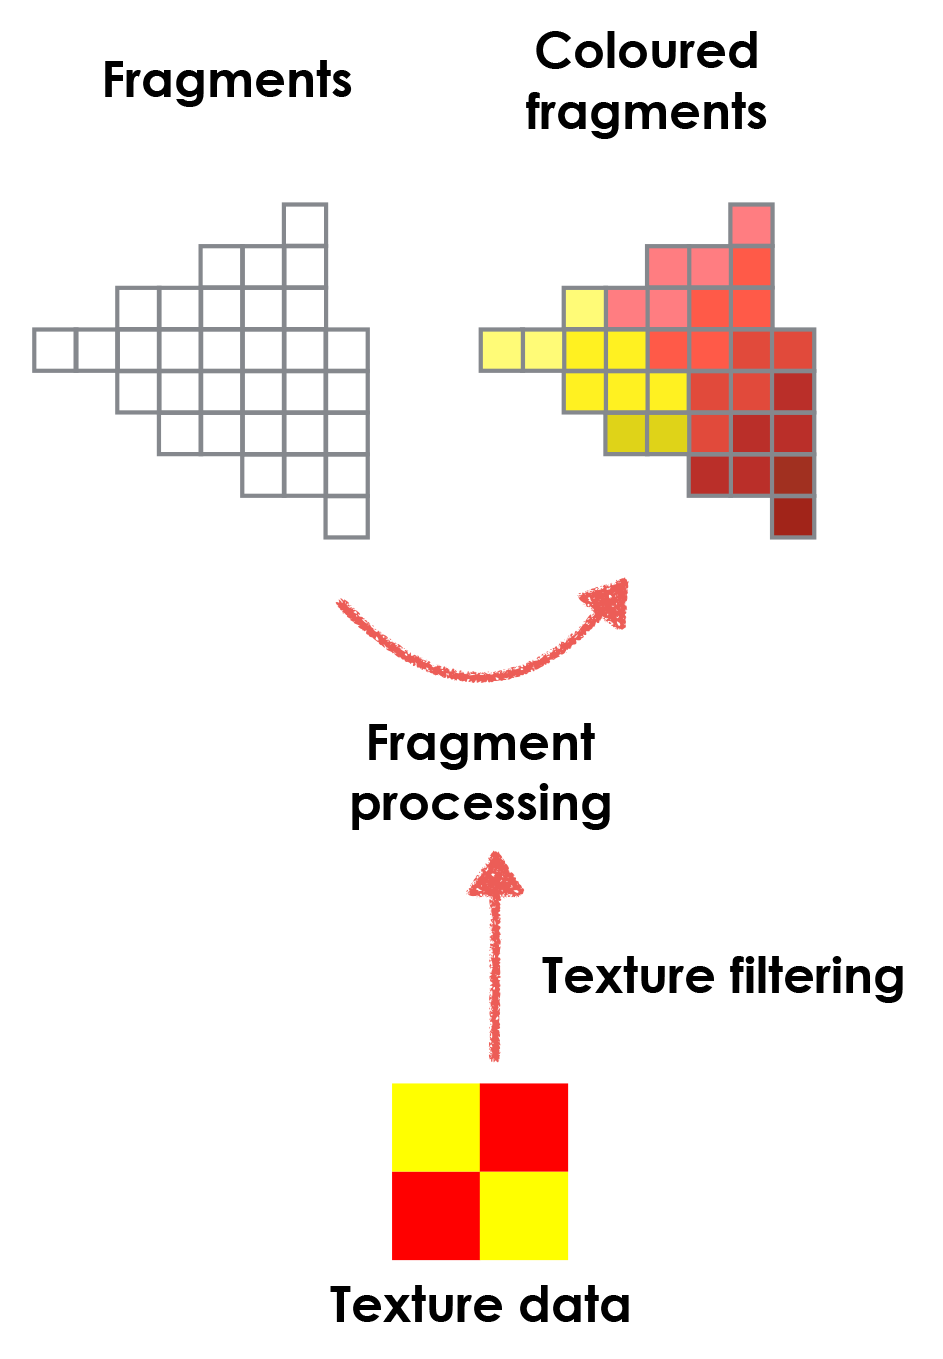
\includegraphics[width=\textwidth]{pipeline_3}
		\end{column}
		\begin{column}{0.65\textwidth}
			\begin{itemize}
				\pause\item Determine the \textbf{colour} of each fragment covered by the triangle
				\pause\item \textbf{Textures} are 2D images that can be \textbf{wrapped} onto a 3D object
				\pause\item Colour is calculated based on \textbf{texture}, \textbf{lighting} and other
					properties of the surface being rendered (e.g.\ shininess, roughness)
			\end{itemize}
		\end{column}
	\end{columns}
\end{frame}

\begin{frame}{Blending}
	\begin{columns}
		\begin{column}{0.3\textwidth}
			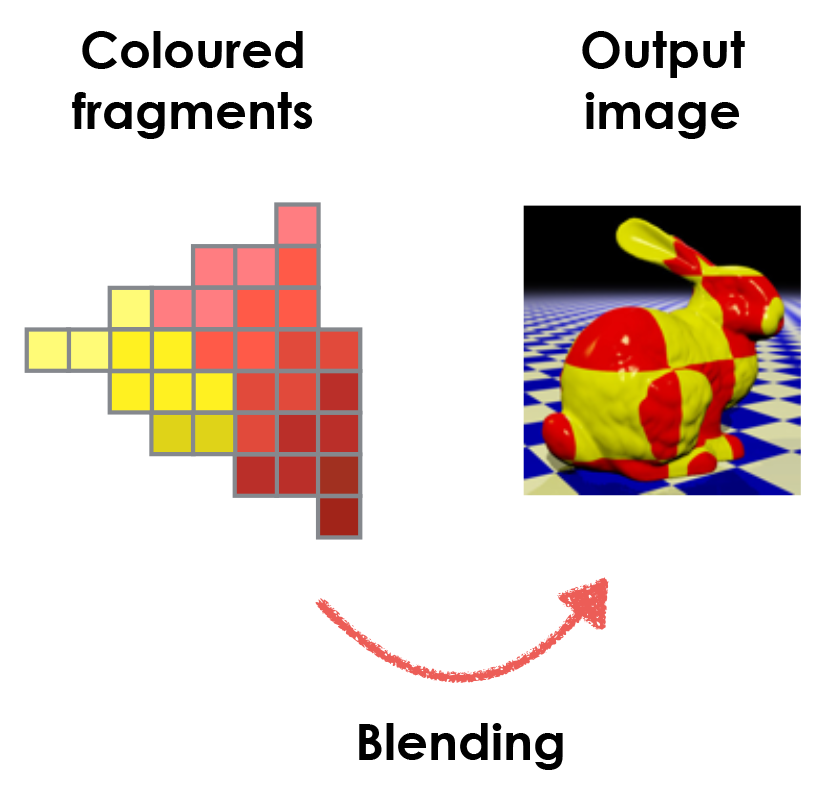
\includegraphics[width=\textwidth]{pipeline_4}
		\end{column}
		\begin{column}{0.65\textwidth}
			\begin{itemize}
				\pause\item Combine these fragments with the existing content of the image buffer
				\pause\item \textbf{Depth testing}: if the new fragment is ``in front'' of the old one, replace it;
					if it is ``behind'', discard it
				\pause\item \textbf{Alpha blending}: combine the old and new colours for a semi-transparent appearance
			\end{itemize}
		\end{column}
	\end{columns}
\end{frame}

\begin{frame}{Shaders}
	\begin{itemize}
		\pause\item The vertex processor and fragment processor are \textbf{programmable}
		\pause\item Programs for these units are called \textbf{shaders}
		\pause\item \textbf{Vertex shader}: responsible for geometric transformations, deformations, and projection
		\pause\item \textbf{Fragment shader}: responsible for the visual appearance of the surface
		\pause\item Vertex shader and fragment shader are separate programs,
			but the vertex shader can pass arbitrary values through to the fragment shader
	\end{itemize}
\end{frame}


\part{GPU Profiling}
\frame{\partpage}

\begin{frame}{Live Demo}
\begin{itemize}
	\pause \item Render Doc
	\pause \item Unity
	\pause \item Unreal 
\end{itemize}
\end{frame}

\part{GPU Optimisation}
\frame{\partpage}

\begin{frame}{Visibility Culling}
\begin{itemize}
	\pause \item You should always cull your scene based on the cameras view fulstrum
	\pause \item This will allow to eliminate objects that are not visible
	\pause \item This combined with a scene graph will allow us to cull large parts of the scene
	\pause \item You should also sort all visible objects from back to front
	\pause \item Caveat, transparent object should be sorted front to back   
\end{itemize}
\end{frame}

\begin{frame}{State Changes}
	\begin{itemize}
		\pause \item You should attempt to minimize state changes
		\pause \item This includes
		\begin{itemize}
			\pause \item Changing Shaders/Materials
			\pause \item Changing Pipeline States
			\pause \item Changing Active Textures
		\end{itemize} 
		\pause \item If you are working in an engine, try to minimum the amount of different materials
		\pause \item This will allow the engine to sort the render queue based on material
		\pause \item Attempt to use a texture atlas to manage your textures
	\end{itemize}
\end{frame}

\begin{frame}{Batching}
	\begin{itemize}
		\pause \item You should attempt to batch your geometry to minimise draw calls
		\begin{itemize}
			\pause \item Unity: Mark GameObject as static
			\pause \item Unreal: Mobility settings, change actors to Static
			\pause \item OpenGL: Have only a few larger VBOs  
		\end{itemize} 
	\end{itemize}
\end{frame}

\begin{frame}{Instancing}
	\begin{itemize}
		\pause \item This allows the GPU to draw one version of the mesh multiple times in one draw call
		\begin{itemize}
			\pause \item Unity: based on materials - Enable Instancing
			\pause \item Unreal: \url{https://forums.unrealengine.com/unreal-engine/events/90518-canon-man-tutorial-hierarchical-instanced-static-meshes-july-26th-live-from-epic-hq?118229=}  
			\pause \item OpenGL: \url{http://www.opengl-tutorial.org/intermediate-tutorials/billboards-particles/particles-instancing/}
		\end{itemize}
	\end{itemize}
\end{frame}

\begin{frame}{Shaders}
	\begin{itemize}
		\pause \item Texture Sampling is one of the biggest source of memory access problems
			\begin{itemize}
				\pause \item Reduce Texture reads
				\pause \item Pack Texture data
				\pause \item Reduce bandwidth by using a 16 bit texture
			\end{itemize}
		\pause \item Avoid branching
			\begin{itemize}
				\pause \item Prefer static branching over dynamic
				\pause \item With static branching, the loop can be evaluated at compile time 
			\end{itemize}
	\end{itemize}
\end{frame}

\end{document}
